





\documentclass[pdflatex,11pt]{aghdpl}
% \documentclass{aghdpl}               % przy kompilacji programem latex
% \documentclass[pdflatex,en]{aghdpl}  % praca w j?zyku angielskim
\usepackage[polish]{babel}
\usepackage[utf8]{inputenc}

% dodatkowe pakiety
\usepackage{enumerate}
\usepackage{listings}
\lstloadlanguages{TeX}



%---------------------------------------------------------------------------

\author{Dorota Wojtałow, Jacek Złydach}
\shortauthor{D. Wojtałów, J. Złydach}
%\shortauthor{M. Szpyrka}

\titlePL{Symulacja rozprzestrzeniania się dymu i ognia w oparciu o niehomogeniczne automaty komórkowe}
\titleEN{Simulation of fire and smoke by using non-homogeous cellular automata}
%\titleEN{Thesis in \LaTeX}


\thesistypePL{Praca inżynierska}

\supervisorPL{dr inż. Jarosław Wąs}
\supervisorEN{Jarosław Wąs Ph.D}

\date{2010}

\facultyPL{Wydział Elektrotechniki, Automatyki, Informatyki i Elektroniki}

\acknowledgements{Serdecznie dziękujemy \dots }

%---------------------------------------------------------------------------

\begin{document}

\titlepages

\tableofcontents
\clearpage

\chapter{Wstęp}
\label{cha:wstep}
%TODO refactoring - czemu nie potrafie zrobić pustej linii przed tezą?!?!?!

%wg. strong Wojnickiego 5 pktow które powinny znaleźć się we wstępie:
% 1. Co - przediot, problem pracy
% 2. Jak - metoda, krotko
% 3. Dlaczego - źrodla problemu badawczego
% 4. Po co - implikacje, konsekwencje, walory
% 5. Co w kolejnych rozdziałach
\section{Temat pracy} % 1 Co

Tematem pracy jest stworzenie symulacji rozprzestrzeniania się dymu i ognia 
w opraciu o niehomogeniczne automaty komórkowe. Zakres pracy obejmuje stworzenie symulacji rozchodzenia się dymu i ognia na podstawie automatów komórkowych wraz z jej wizualizacją, a także walidację stworzonego modelu. 
Celem pracy jest pokazanie możliwości niehomogenicznych automatów komórkowych jako narzędzia umożliwiającego 
odzwierciedlenie rzeczywistego rozprzestrzeniania się dymu i ognia podczas pożaru. 

\section {Geneza tematu} %3 i 4 - Dlaczego i po co

W dobie wszechobecnej urbanizacji i ciągłego budownictwa, wraz ze wzrostem świadomości dotyczącej bezpieczeństwa
pożarowego oraz zaangażowania w jego zagwarantowaniu pojawiła się potrzeba możliwości modelowania i obserwacji rozprzestrzeniania się ognia w zamkniętych budynkach.
Wspomniane symulacje pożarów wykazują szereg zastosowań. Są z powodzeniem wykorzystywane w śledztwach. Dają możliwość odtworzenia przebiegu zdarzeń i porównania z wynikami oględzin. Umożliwiają
zbadanie prototypu budynku pod kątem gwarancji bezpieczeństwa pożarowego. 
Ułatwiają projektowanie systemów oddymiania. W połączeniu z modelami ewakuacji ludzi
stanowią kompleksowy system ułatwiający tworzenie bezpiecznych budowli.

W ostatnich latach powstał szereg programów umożliwiających wizualizcję symulacji rozchodzenia ognia. Opracowane dotychczas rozwiązania swoje działanie 
opierają na metodach numerycznej dynamiki płynów (ang. Computational Fluid Dynamics). Niewątpliwą zaletą numerycznego podejścia jest dokładność wyników. 
Głównymi wadami jest złożoność obliczeń i stopień komplikacji modelu. 
Niehomogeniczne automaty komórkowe umożliwiają znaczne uproszczenie modelu. Uproszczenie modelu powoduje z kolei redukcję złożoności
obliczeń czyniąc automaty komórkowe szczególnie dogodną metodą w przypadku tworzenia prototypów oraz symulacji czasu rzeczywistego.

%dopisać coś jeszcze o tym, że nie ma takich symulatorów wyk. automaty komórkowe 



\textbf{Teza} Wykorzystując zasady tworzenia automatów komórkowych oraz w oparciu o prawa fizyki można w realistyczny sposób
przy użyciu niehomogenicznych 
automatów komórkowych
zamodelować zjawiska rozchodzenia się ognia i dymu podczas pożaru.

W celu wykazania powyższej tezy przeprowadzono następujące działania:
\begin{itemize}
\item Przeprowadzono badania dotyczące zjawisk fizycznych zachodzących podczas pożaru.
\item Zidentyfikowano czynniki mające kluczowy wpływ na kształt i charakter pożaru.
\item Zaproponowano model niehomogenicznego automatu komórkowego odzwierciedlającego prawa fizyczne.
\item Zaimplementowano opracowany algorytm wraz z wizualizacją wyników oraz możliwością edycji danych wejściowych oraz kontroli symulacji w czasie rzeczywistym.
\item Dokonano weryfikacji jakościowej zaproponowanego modelu.
\end{itemize}

\section {Realizacja projektu} % 2 - jak
Praca została zrealizowana jako wolnostojąca aplikacja komputerowa napisana w języku Java. Do renderowania grafiki trójwymiarowej
zostala użyta biblioteka graficzna Java3D. Aplikacja została przetestowana z wykorzystaniem biblioteki JUnit4. 

\section{Zawartość pracy} % 5 - co w kolejnych rozdziałach Tutaj na pewno trzeba dać odnośniki do rozdziałów a nie tytuły!
Praca składa się z [iluś] rozdziałów. 
W pierwszym rozdziale znajdują się podstawy teoretyczne, związane zarówno z modelowanymi zjawiskami fizycznymi jak i użytym algorytmem.
Rozdział Modele symulacji zawiera propozycje zweryfikowanych modeli rozprzestrzeniania się dymu i ognia zaprojektowanych w oparciu
o niehomogeniczne automaty komórkowe. Rozdział Implementacja przedstawia sposób realizacji projektu, napotkane problemy oraz 
ich rozwiązania. Opisuje możliwości graficznego interfejsu użytkownika oraz sposób korzystania z niego.
 % W podsumowaniu znajduje się podsumowanie.... nie wiem jeszcze jak to ładnie ująć
%cos wiecej o rozdzialach. dopisac jak będa gotowe

%TODO:
%Wstawić rysunek konwekcji narysowany ze screena z Rosenbajgerowymi strzałkami
%Konwekcja, a grawitacja i prawo Archimedesa
\chapter{Teoria}
\label{cha:Teoria}
Kluczowym elementem, niezbędnym do prawidłowego zamodelowania pożaru
jest zrozumienie czym jest ogień oraz poznanie zjawisk jakim podlega. Niniejszy rozdział zawiera
krótki wstęp teoretyczny, przedstawiający zjawiska fizyczne niezbędne do zrozumienia istoty 
pożaru i prawidłowego jego zamodelowania.
\section {Czym jest ogień}
Ogień nie jest substancją.
Ogień powstaje jako produkt reakcji chemicznej zachodzącej między paliwem i tlenem.
Obserwowalną postać ognia, czyli to co widzimy i nazywamy ogniem tworzy światło powstałe w wyniku ruchu rozgrzanego powietrzna.
Jest to jednak tylko jeden z aspektów tego złożonego procesu.
Elementami koniecznymi do powstania i podtrzymania ognia są:
\begin{itemize}
\item tlen
\item paliwo
\item ciepło
\end{itemize}


Paliwem może być ciecz, ciało stałe lub gaz. Samo w sobie paliwo nie ulega spalaniu. 
Paliwo pod wpływem ciepła pochodzącego np. z zapałki lub otrzymanego od innego nagrzanego ciała ogrzewa się. Po osiągnięciu
odpowiedniej temperatury, paliwo ulega procesowi dekompozycji. Jednym z produktów dekompozycji
są opary. W przypadku jednego z najbardziej popularnych paliw - drewna oprócz oparów w wyniku dekompozycji otrzymujemy węgiel i popiół.
Spalanie drewna przedstawia poniższa reakcja \ref{reakcja_spalania}:
\begin {equation}
CH_2O+O_2+heat ->CO_2 + CO + C + N_2 + H_2O
\label {reakcja_spalania}
\end {equation}
Kiedy opary osiągną odpowiednią temperaturę tzw. temperaturę zapłonu (w przypadku drewna wynosi ona ok. $300^\circ C$) oraz gdy ich stężenie
w powietrzu jest odpowiednie może dojść do zapłonu. Do zapłonu dochodzi w wyniku kontaktu z otwartym ogniem, iskrą lub w wyniku osiągnięcia
przez opary temperatury tzn. samozapłonu. Wynikiem zapłonu jest spalanie oparów. Jak widać głównym substratem reakcji spalania są opary powstające w wyniku
ogrzania paliwa. W przypadku niektórych paliw jest to jedyny reagent. Jednym z przykładów jest benzyna, która w wyniku ogrzania w całości zamienia się w opary ulegające spalaniu. W przypadku drewna, poza oparami spalaniu ulega także węgiel. Jest to jednak reakcja bardzo powolna.
Na szczególną uwagę zasługuje fakt wytwarzania energii cieplnej w procesie spalania, co powoduje samoistne podtrzymanie ognia. Płomień będący
wizualną postacią spalania ogrzewa sąsiadujące cząsteczki paliwa, dzięki czemu nie gaśnie.

Bardzo istotnym reagentem w procesie spalania jest tlen. Atomy gazów, oparów powstałych w wyniku podgrzania paliwa w wyniku zapłonu łączą się z tlenem.
Aby mogło dojść do reakcji spalania bardzo ważne jest zachowanie odpowiednich proporcji między substratami reakcji. Lower Explosive Limit (LEL) określa 
minimalne stężenie oparów w powietrzu, konieczne aby mogło dojść do zapłonu. Odpowiednio, Upper Explosive Limit (UEL) oznacza maksymalne stężenie oparów, powyżej
którego nie dojdzie do zapłonu. Przykładowo: dla tlenku węgla $LEL=12$, natomiast  $UEL=75$, co oznacza w powietrzu musi być między $12\%-75\%$ aby mogło dojść
do jego zapalenia. $LEL$ oraz $UEL$ określają także pośrednio wymaganą ilość tlenu. Dla większości paliw ilość tlenu wymaganego do zapłonu wynosi ok. $15\%$. 

\section {Propagacja ciepła}
Jak zostało wspomniane w rozdziale \ref{Proces spalania} jednym z czynników niezbędnych
do podtrzymania ognia jest ciepło. Ciepło podczas pożaru jest propagowane na trzy różne sposoby:
\begin {itemize}
\item Przewodnictwo
\item Konwekcja
\item Radiacja
\end {itemize}

\subsection {Przewodnictwo}
\label{Przewodnictwo}
 Przewodnictwo cieplne jest procesem, który polega  na wymianie ciepła 
pomiędzy nierównomiernie ogrzanymi ciałami będącymi w kontakcie. Zachodzi ono we wszystkich stanach skupienia: ciałach stałych, cieczach i gazach, jednak sposób i skala tego zjawiska jest bardzo zróżnicowana. Najczęściej mówimy o przewodnictwie w ciałach stałych.
W cieczach i gazach występuje ono niezmiernie rzadko i polega na zderzeniach cząsteczek podlegających
niezorganizowanym, przypadkowym ruchom i ich dyfuzji.
W ciałach stałych przenoszenie ciepła odbywa się  na dwa sposoby:
\begin{itemize}
\item dzięki drganiom atomów
\item poprzez ruch elektronów
\end {itemize}
Celem omawianego przewodnictwa jest 
osiągnięcie równowagi cieplnej. Podczas przewodnictwa ciepło jest zawsze przenoszone od
ciała o większej temperaturze do ciała o niższej. Zgodnie z zasadą zachowania energii, głoszącą że w układzie 
izolowanym suma wszystkich energii jest stała, ilość energii uzyskanej przez ciało chłodniejsze jest równa
ilości energii oddanej przez cieplejszy obiekt. Energia przenoszona jest wraz z ruchem cząsteczek wewnętrznych.
Nie wszystkie ciała przewodzą ciepło w takim sam sposób.
Zależność między ilością ciepła przewodzonego przez ciało, a jego zmianą temperatury najlepiej opisuje prawo Fouriera.
Przyjmuje ono następującą postać:
\begin{equation}
 q(r,t)=-k*grad T
 \label{eqn:fourier}
\end {equation}
gdzie:
k - współczynnik przewodzenia ciepła $[W / (m*K)]$
T - temperatura $[K]$
q - natężenie strumienia ciepła  $[W/(m^2)]$
Prawo Fouriera oznacza, że gęstość strumienia ciepła przekazywana w jednostce czasu przez jednostkową powierzchnię 
jest proporcjonalna do gradientu temperatury. Minus we wzorze wynika ze wspominanego wyżej kierunku przepływu ciepła:
od ciała cieplejszego do zimniejszego. Strumień ciepła jest mierzony w kierunku zgodnym z jego przepływem, zatem przyrost
temperatury będzie miał wartość ujemną.


Do dobrych przewodników należą przede wszystkim:
\begin {itemize}
\item metale - do najlepszych należą srebro, miedź, złoto, aluminium
\end {itemize}
Źle przewodzą ciepło:
\begin {itemize}
\item drewno
\item papier
\item ciecze
\item gazy
\end {itemize}
Zła przewodność cieczy i gazów wynika z istoty procesu przewodnictwa w tych stanach skupienia. Za wysoką wartość 
współczynnika przewodnictwa odpowiada ruch elektronów. Dlatego też, we wszystkich dialektrykach wartość ta
przyjmuje wartości z przedziału $[0,001-3][W/(m*K)]$, podczas gdy w metalach może sięgać ona nawet $ 400 [W/m*k]$

Na uwagę zasługuje też fakt, że przewodność metali maleje wraz ze wzrostem ich temperatury.
Tabela \ref {przewodnictwa} zawiera współczynniki przewodnictwa przykładowych materiałów, które zostały wykorzystane przy
testowaniu algorytmu symulacji.
%http://tabelechemiczne.chemicalforum.eu/przewodnictwo_ciala.html
%Dodać do bibliografii tablice fizyczne z których to wzięte
\begin{table}
\begin {center}
\begin{tabular} {|l | c | c|}
\hline
Materiał & Temp. $[C]$ & Wspł. przewodnictwa $[W/(m*K)]$ \\ \hline
Beton & 20 & 0.84-1.3  \\ \hline
Drewno & - & 0.1-0.17  \\ \hline
Szkło crown & 20 & 0.22-0.29  \\ \hline
Azbest & 20 & 0.16-0.37 \\ \hline
Guma wulkanizowana & 20 & 0.22-0.29 \\ \hline
Miedź & 20 & 400 \\ \hline
Stal & 20 & 10 \\ \hline
Ołów & 20 & 30 \\ \hline
Powietrze & 20 & 0.025 \\ 
\hline
\end {tabular}
\caption{Współczynniki przewodnictwa materiałów}
\label{przewodnictwa}
\end{center}
\end {table}
\subsection{Konwekcja}
\label{Konwekcja}
Konwekcja, zwana też unoszeniem lub wnikaniem jest to zgodnie ze szkolną definicją sposób przewodnictwa ciepła polegający na
"unoszeniu pobranej energii cieplnej przez cząsteczki substancji i dzięki swojej wędrówce przekazywaniu
energii innym cząsteczkom". 
jak się znajdzie jakaś inna przystępna definicja to podmienić
Konwekcja zachodzi we wszystkich płynach, czyli zarówno cieczach jak i gazach. Nie zachodzi natomiast w ciałach stałych.
Konwekcja ze względu na połączenie w sobie dwóch zjawisk: 
\begin{itemize}
\item przekazywania ciepła
\item ruchu płynów
\end{itemize}
jest zjawiskiem niezwykle skomplikowanym do teoretycznego ujęcia. Przenoszenie ciepła w konwekcji zachodzi 
wskutek ruchu płynu, tak więc warunkiem niezbędnym do wystąpienia zjawiska konwekcji jest ruch ośrodka.
Można wyróżnić dwa podstawowe typy konwekcji, dzielące zjawisko wnikania ze względu na przyczynę ruchu ośrodka:
\begin{itemize}
\item konwekcja naturalna - w tym przypadku ruch płynu wywołany jest różnicami gęstości substancji znajdujących się w polu grawitacyjnym
\item konwekcja wymuszona - ruch płynu spowodowany jest działaniem urządzeń zewnętrznych (wentylatorów, pomp)
\end {itemize}
Przykładem konwekcji naturalnej jest unoszenie ciepłego powietrzna w pomieszczeniu. 
Ogrzane powietrze zmniejsza swoją gęstość, w wyniku czego unosi się do góry. Jego miejsce wypełnia zimne powietrze, 
które w kolejnym etapie ulega ogrzaniu rozpoczynając kolejny cykl wędrówki powietrza. Ruchy powietrza wywołane zjawiskiem 
konwekcji tworzą tzw. prądy konwekcyjne.
%TODO dodać rysunek konwekcji
 Konwekcja naturalna jest typem konwekcji występującym podczas pożaru. 

\subsection {Radiacja}
\label{Radiacja}
Radiacja, czyli inaczej promieniowanie jest to sposób rozchodzenia ciepła w postaci fal elektromagnetycznych. 
Najważniejszym aspektem przewodnictwa ciepła przez promieniowanie jest możliwość wymiany ciepła między ciałami
nie stykającymi się.
W bardzo niskich temperaturach ilość przekazywanego przy pomocy radiacji ciepła jest tak mała, że zjawisko to może być pomijane.
Wzrost znaczenia promieniowania następuje wraz ze wzrostem temperatury ciał wymieniających ciepło.
Przyjmuje się, że radiacja zachodzi dla ciał o temperaturach wyższych od $0 ^\circ$ Kelvin.
Promieniowanie jest rodzajem wymiany energii, która nie wymaga żadnego nośnika. Każde ciało emituje fale.
W normalnych warunkach większość promieniowania zachodzi przy udziale fal podczerwonych. Należy jednak pamiętać
że w radiacji mogą brać udział także fale świetlne czy ultrafioletowe. Poza emisją promieniowania każde ciało reaguje także
na fale wysyłane przez innych. Dla każdego ciała jesteśmy w stanie określić wartości trzech współczynników opisujących 
reakcję ciała na wiązkę promieniowania. Należą do nich:
\begin {itemize}
\item Absorpcyjność czyli pochłanialność
\item Refleksyjność czyli odbijalność
\item Przepuszczalność
\end {itemize}
Radiacja następuje we wszystkich kierunkach aż  do momentu zablokowania drogi promieni przez ciało pochłaniające je.
Większość ciał stałych o rozmiarach większych od kilku mikrometrów nie przepuszcza promieniowania. Na wspomnianej 
głębokości pod powierzchnią ciała następuje całkowita absorpcja promieniowania cieplnego. Ponadto ciała stałe mogą przepuszczać
fale tylko o określonej długości. Przykładem jest szkło, które przepuszcza jedynie fale świetlne.
Ilość promieniowania emitowanego przez ciała szare można obliczyć ze wzoru \ref{emisyjnosc}
\begin {equation}
\dot{Q_{emit}}=\sigma*\varepsilon*A_{s}*T_{s}^4
\label {emisyjnosc}
\end {equation}
gdzie
\begin{itemize}
\item $\varepsilon \in (0,1)$ - emisyjność powierzchni. $\varepsilon=1$ - dla ciała doskonale czarnego. Określa jak bardzo dane 
ciało jest podobne do ciała doskonale czarnego.
\item $\sigma = 5.67 * 10^-8 [W/(m^2 * K^4]) $ - stała promieniowania
\item $A_{s} [m^2]$ - powierzchnia 
\item $T_{s} [K]$ - temperatura
\end {itemize}
Przeanalizujmy przykład promieniowania między rzeczywistymi obiektami znajdującymi się w pewnym pomieszczeniu np. stół w pokoju.
W przypadku jednej powierzchni zamkniętej w innej (w omawianym przypadku wewnętrzną powierzchnią będzie powierzchnia stołu, natomiast zewnętrzną ściany pokoju) zakłada się, że wewnętrzna powierzchnia "nie opromieniowuje samej siebie".
Innymi słowy całe promieniowania ciała wewnętrznego przechodzi do powierzchni zewnętrznej. W drugim kierunku następuje tylko częściowe
przejście energii z ciała zewnętrznego do wewnątrz. Ponadto, w przypadku gdy otaczająca powierzchnia jest znacząco większa od powierzchni wewnętrznej i obie powierzchnie są oddzielone gazem, który nie promieniuje (powietrze) zjawisko promieniowania zachodzi
równolegle ze zjawiskiem konwekcji i oba te zjawiska należy wziąć pod uwagę równocześnie.
W takim przypadku wymianę ciepła można określić za pomocą wzoru \ref{emisyjnosc_konwekcja}
\begin {equation}
\dot{Q_{całk}}=\alfa_{całk}*\sigma*A_{s}*(T_{s}^4-T_\inf^4)
\label {emisyjnosc_konwekcja}
\end {equation}
gdzie:
\begin {itemize}
\item \alfa_{całk} - całkowity współczynnik wymiany ciepła
\item T_\inf - temperatura powietrza w znacznej odległości
\end {itemize} 
Omówione powyżej procesy powodują, że promieniowanie jest zjawiskiem szczególnie skomplikowanym.

\subsection {Zależność temperatury od dostarczonej energii}
Opisane w podrozdziałach \ref{Przewodnictwo}, \ref{Konwekcja}, \ref{Radiacja} metody obrazują różne sposoby przekazywania energii
między cząsteczkami materii. Po ich poznaniu należy zadać sobie pytanie w jaki sposób ta energia wpływa na temperaturę substancji?
Wielkością reprezentującą zależność między dostarczoną energią a temperaturą substancji jest ciepło właściwe. Ciepło właściwe
jest wielkością charakterystyczną dla materiału i  informuje ono o tym ile ciepła
należy dostarczyć aby ograć 1kg substancji o $1^\circ C$.Opisaną powyżej zależność przedstawia wzór \ref{cieplo_wlasciwe} 
\begin {equation}
c=Q/(m*\Delta T)
\label {cieplo_wlasciwe}  
\end {equation}
gdzie:
\begin {itemize}
\item c - ciepło właściwe $[J/ (kg * K)]$
\item m - masa ciała $[kg]$
\item T - temperatura  $[K]$
\end {itemize}
Znając ilość ciepła dostarczonego do ciała w wyniku procesów przekazywania energii oraz dokonując przekształcenia powyższego wzoru
można w bardzo prosty sposób policzyć zmianę temperatury badanego ciała.


\chapter {Projekt}
\label{cha:projekt}
\section {Główne zalożenia}
\begin {itemize}
\item Głównym celem projektu jest stworzenie i weryfikacja modelu rozprzestrzeniania się ognia wykorzystując niehomogeniczne automaty
komórkowe. Nacisk z pracy został położony na opracowanie algorytmu najdokładniej oddającego rzeczywistość.
\item Projekt obejmuje także swtworzenie uproszczonej wizualizacji symulacji oraz graficznego interfejsu użytkownika (GUI).
\item Interfejs aplikacji powinien umożliwiać edycję budynku w którym przeprowadzana jest symulacja: dodawanie elementów konstrukcji, 
określanie materiałów z których zostały stworzone. 
\item Użytkownik powinien mieć możliwość określenia źródła ognia: zarówno jego miejsca jak i temperatury początkowej.
\item Aplikacja powinna umożliwiać także kontrolę nad symulacją: możliwość zatrzymania symulacji, wznowienia, rozpoczęcia od początku,
a także dostosowanie tempa symulacji umożliwiającego obserwację zjawisk fizycznych.
\end {itemize}
\section {Architektura aplikacji}
% w bibliografi powinno byc coś o tej architekturze i def. aktywnego modelu
Aplikacja została zaprojektowana zgodnie z architekturą Model-View-Controller.
Poniższy schemat przedstawia typowy przykład architektury Model-View-Controller:
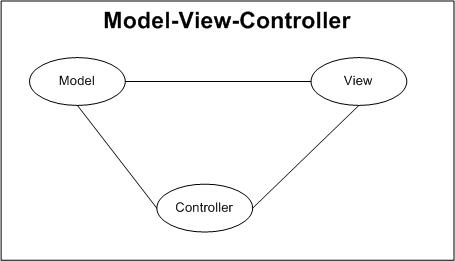
\includegraphics{MVC.jpeg}
W omawianej pracy została zaimplementowana pewna odmiana typowej architektury Model-Widok-Kontroler.
Najodpowiedniej przedstawia ją poniższy rysunek:
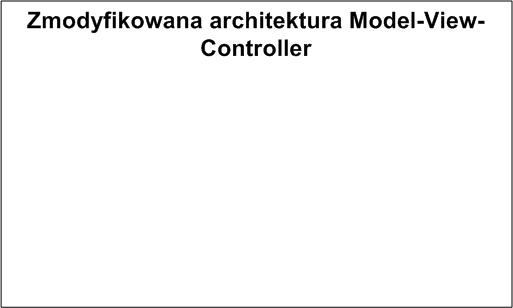
\includegraphics{modifiedMVC.jpeg}
Kontroler odpowiada za pobranie danych od użytkownika, ich przetworzenie oraz dostarczenie do modelu.
Został zastosowany przypadek aktywnego modelu, który zgodnie z definicją potrafi zmieniać swój stan 
bez względu na akcje wykonywane przez użytkownika. W projekcie symulacji pożaru aktywność modelu polega na 
wykonywaniu pętli symulacji, związanych z nią obliczeń, powiadamianiu widoku o zachodzących zmianach oraz
końcu symulacji. Widok odpowiada jedynie za prezentację wyników symulacji.
Wybrana architektura umożliwia elastyczny rozwój aplikacji. Wprowadzony podział na trzy odrębne moduły pozwala
na nieograniczone zmiany w każdym z nich, nie powodując konieczności zmian innych części aplikacji.
Inną zaletą separacji jest łatwość testowania poszcególnych modułów osobno. 
\section {Moduły}
\section {Obiekty}

% itd.
% \appendix
% \include{dodatekA}
% \include{dodatekB}
% itd.

\bibliography{bibliografia}

\end{document}

